\documentclass[border=14pt,tikz]{standalone}
\usepackage{fontspec}
\setmainfont{Helvetica Neue}
\setsansfont{Helvetica Neue}
\setmonofont{Menlo}
\usepackage{amsmath}
\usepackage{tikz}
\usetikzlibrary{positioning, arrows.meta}

\definecolor{kernel}{HTML}{E3F2FD}
\definecolor{kernelborder}{HTML}{2196F3}
\definecolor{state}{HTML}{E8F5E9}
\definecolor{stateborder}{HTML}{4CAF50}
\definecolor{choice}{HTML}{FFF3E0}
\definecolor{choiceborder}{HTML}{FF9800}

\begin{document}
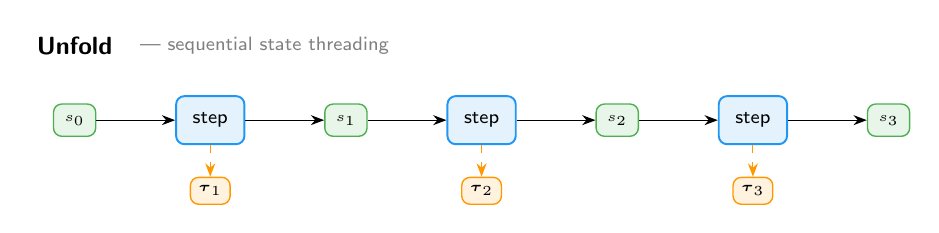
\begin{tikzpicture}[
    >=Stealth,
    node distance=0.8cm and 1cm,
    kern/.style={draw, rounded corners=3pt, inner sep=6pt,
                 font=\sffamily\scriptsize, fill=kernel, draw=kernelborder, line width=0.7pt},
    st/.style={draw, rounded corners=3pt, inner sep=4pt,
               font=\ttfamily\tiny, fill=state, draw=stateborder, line width=0.5pt},
    ch/.style={draw, rounded corners=3pt, inner sep=3pt,
               font=\ttfamily\tiny, fill=choice, draw=choiceborder, line width=0.5pt},
    title/.style={font=\sffamily\small\bfseries},
    annot/.style={font=\sffamily\scriptsize, text=black!50},
]

\node[title] (ut) {Unfold};
\node[annot, right=3pt of ut] {--- sequential state threading};

\node[st, below=0.5cm of ut] (s0) {$s_0$};
\node[kern, right=of s0] (k1) {step};
\node[st, right=of k1] (s1) {$s_1$};
\node[kern, right=of s1] (k2) {step};
\node[st, right=of k2] (s2) {$s_2$};
\node[kern, right=of s2] (k3) {step};
\node[st, right=of k3] (s3) {$s_3$};

\draw[->] (s0) -- (k1);
\draw[->] (k1) -- (s1);
\draw[->] (s1) -- (k2);
\draw[->] (k2) -- (s2);
\draw[->] (s2) -- (k3);
\draw[->] (k3) -- (s3);

\node[ch, below=0.4cm of k1] (c1) {$\boldsymbol{\tau}_1$};
\node[ch, below=0.4cm of k2] (c2) {$\boldsymbol{\tau}_2$};
\node[ch, below=0.4cm of k3] (c3) {$\boldsymbol{\tau}_3$};
\draw[->, dashed, choiceborder] (k1) -- (c1);
\draw[->, dashed, choiceborder] (k2) -- (c2);
\draw[->, dashed, choiceborder] (k3) -- (c3);

\end{tikzpicture}
\end{document}
